\clearpage

\section{Results}

In this section we provide the results of the inclusive and targeted searches. The observed and predicted \MET\ distributions for the
inclusive analysis are indicated in Fig.~\ref{fig:results_incl}. A summary of the results in the signal regions is provided in
Table~\ref{tab:results_incl}. Currently we blind the observed data yields for the signal regions, defined by \MET\ $>$ 100 GeV.
These yields will be presented when the decision is made to unblind the Z region for the Aachen/ETH low-mass opposite-sign same-flavor
dilepton analysis (``edge analysis''). In the low \MET\ region, we observe good agreement between the data and the predicted background,
which validates the background estimation methodology.
The separate results for the ee and $\mu\mu$ channels are presented in App.~\ref{app:results}.

\begin{figure}[!h]
\begin{center}
\begin{tabular}{cc}
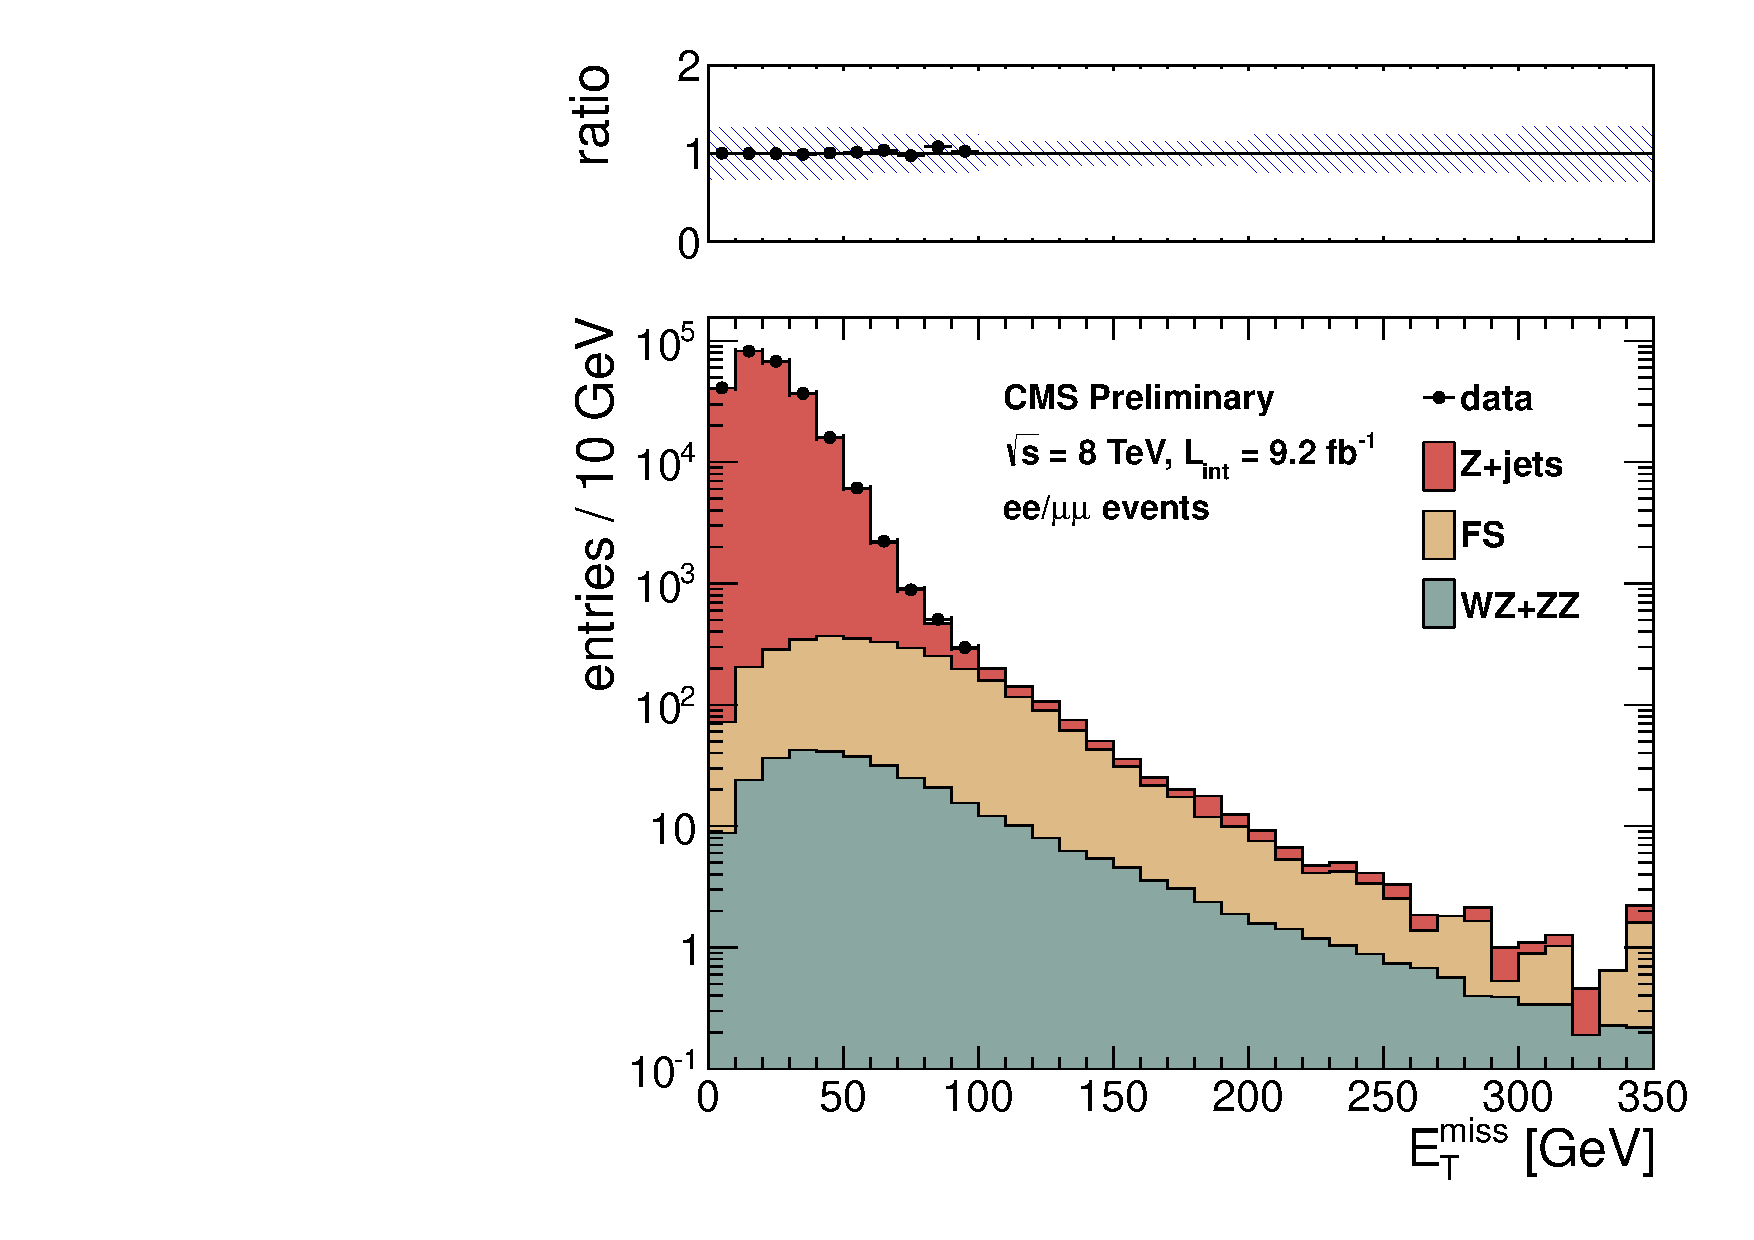
\includegraphics[width=0.6\textwidth]{plots/pfmet_all_92fb.pdf}
\end{tabular}
\caption{Results of the inclusive analysis. The observed \MET\ distribution (black points) is compared with the sum of the predicted \MET\
distributions from \zjets, flavor-symmetric backgrounds, and WZ+ZZ backgrounds. The ratio of observed to predicted yields in each bin is
indicated. The error bars indicate the statistical uncertainty in the data and the shaded band indicates the total background uncertainty.
\label{fig:results_incl}
}
\end{center}
\end{figure}



\begin{table}[htb]
\begin{center}
\footnotesize
\caption{\label{tab:results_incl} Summary of results in the inclusive analysis. The total background is the sum of the \zjets\ background predicted from
the \MET\ templates method (\zjets\ bkg), the flavor-symmetric background predicted from e$\mu$ events (FS bkg), and the WZ and ZZ backgrounds predicted from MC
(WZ bkg and ZZ bkg). All uncertainties include both the statistical and systematic components. The Gaussian significance of the deviation between the data 
and total background is indicated for signal regions with at least 20 observed events. }
\begin{tabular}{l|c|c|c|c|c|c}

\hline
\hline
                      &   \MET\ 0--30 GeV   &  \MET\ 30--60 GeV   & \MET\ 60--100 GeV   &\MET\ 100--200 GeV   &\MET\ 200--300 GeV   & \MET\ $>$ 300 GeV  \\
\hline
        \zjets\ bkg   &190124 $\pm$ 57038   & 57993 $\pm$ 17399   &    2744 $\pm$ 824   &      123 $\pm$ 37   &     7.4 $\pm$ 2.4   &     1.3 $\pm$ 0.5  \\
             FS bkg   &      492 $\pm$ 77   &     947 $\pm$ 147   &     981 $\pm$ 152   &      503 $\pm$ 78   &    23.6 $\pm$ 7.1   &     3.0 $\pm$ 1.9  \\
             WZ bkg   &   61.5 $\pm$ 43.0   &  104.8 $\pm$ 73.4   &   75.4 $\pm$ 52.8   &   41.2 $\pm$ 28.8   &     5.6 $\pm$ 3.9   &     1.6 $\pm$ 1.6  \\
             ZZ bkg   &     7.6 $\pm$ 3.8   &    16.2 $\pm$ 8.1   &    17.4 $\pm$ 8.7   &    16.1 $\pm$ 8.1   &     3.2 $\pm$ 1.6   &     1.0 $\pm$ 1.0  \\
\hline
          total bkg   &190685 $\pm$ 57038   & 59061 $\pm$ 17400   &    3818 $\pm$ 840   &      683 $\pm$ 92   &    39.9 $\pm$ 8.6   &     6.9 $\pm$ 2.7  \\
               data   &            190793   &             58953   &              3921   &                 ?   &                 ?   &                 ?  \\
       significance   &               0.0   &              -0.0   &               0.1   &                 ?   &                 ?   &                 ?  \\
\hline
\hline
\end{tabular}
\end{center}
\end{table}

\clearpage

The observed and predicted \MET\ distributions for the targeted analysis are indicated in Fig.~\ref{fig:results_targ}. A summary of the 
results in the signal regions is provided in Table~\ref{tab:results_targ}. 
Here the results in the signal regions with \MET $>$ 100 GeV region are also blinded, pending completion of signal optimization studies
(see Sec.~\ref{sec:optimization}).
The observed yields are in good agreement with the predicted background the low \MET\ region, validating the background estimation
methodology.

\begin{figure}[!h]
\begin{center}
\begin{tabular}{cc}
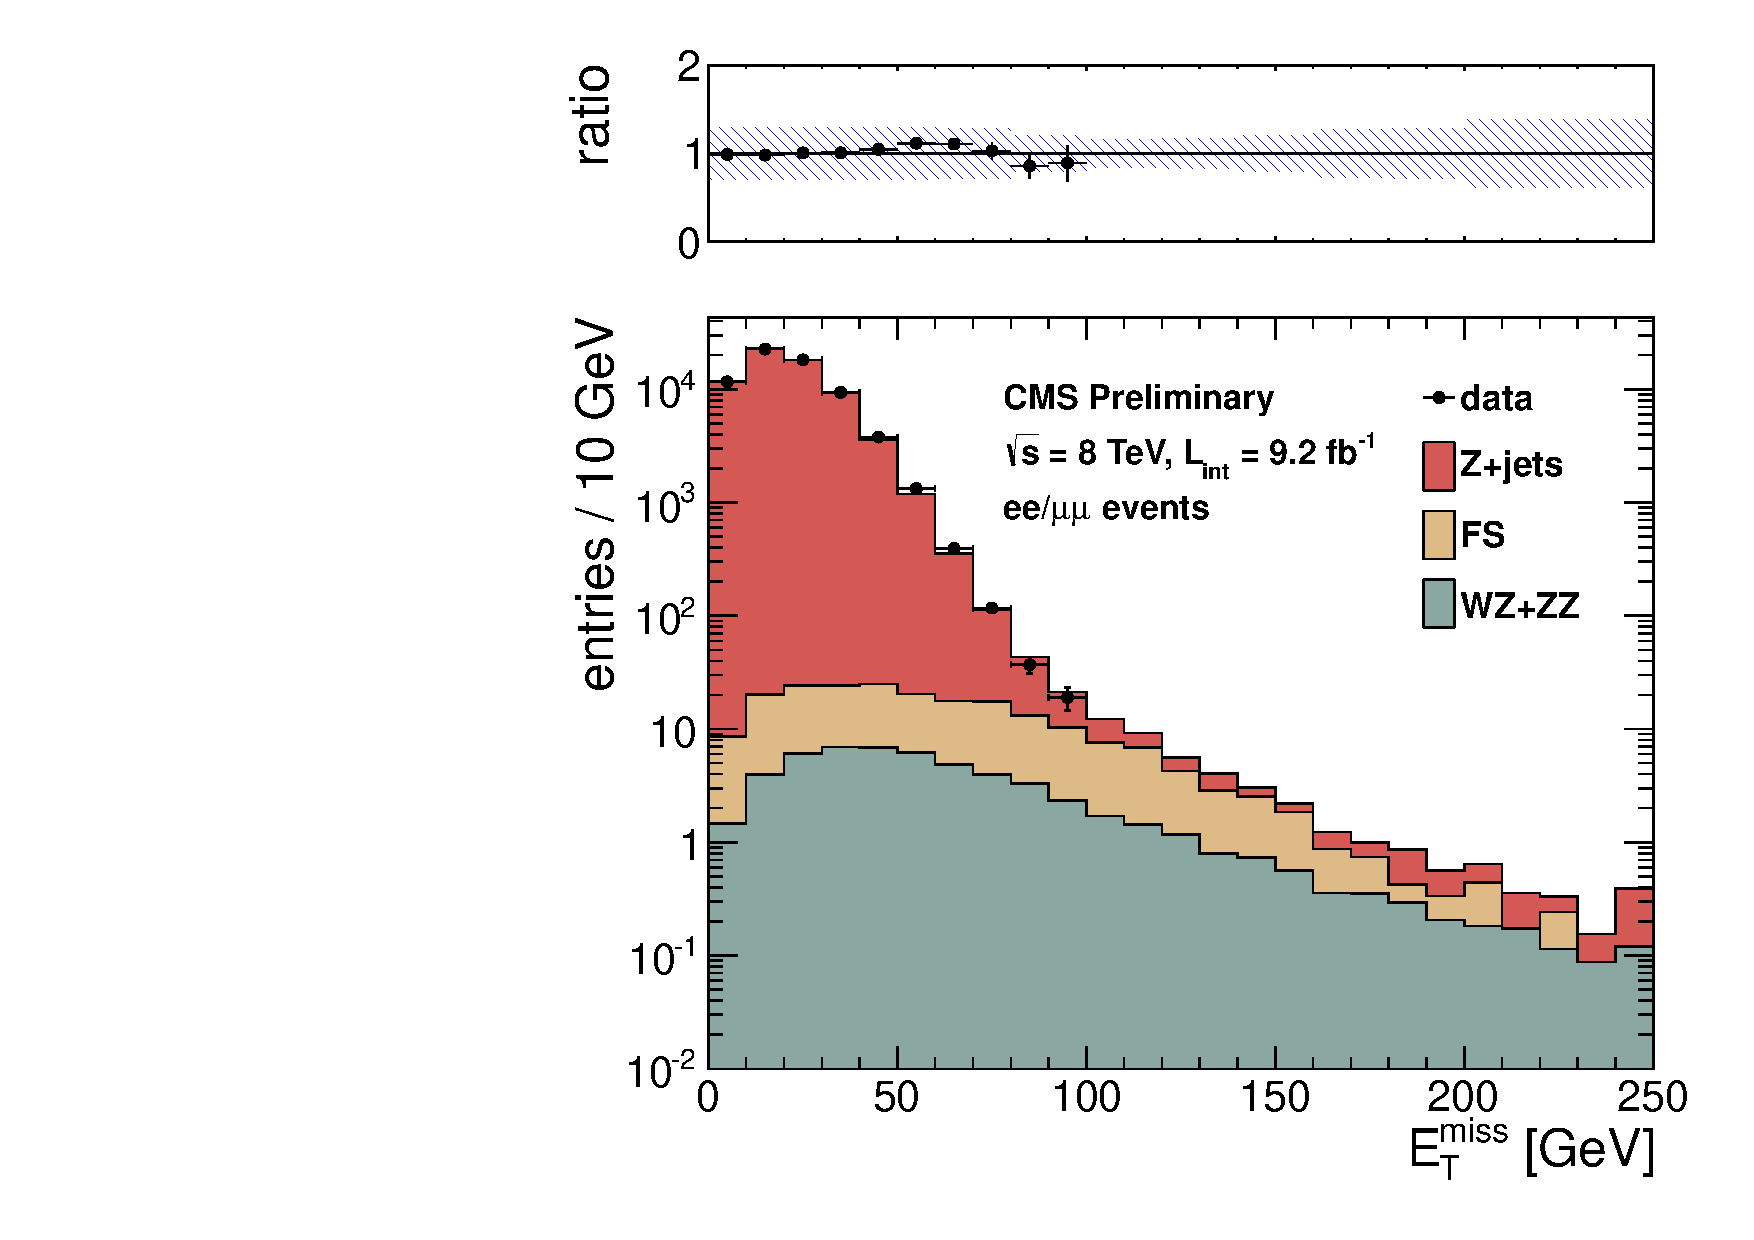
\includegraphics[width=0.5\textwidth]{plots/pfmet_bvetoMedium_all_92fb.pdf}
\end{tabular}
\caption{Results of the targeted analysis. The observed \MET\ distribution (black points) is compared with the sum of the predicted \MET\
distributions from \zjets, flavor-symmetric backgrounds, and WZ+ZZ backgrounds. The ratio of observed to predicted yields in each bin is
indicated. The error bars indicate the statistical uncertainty in the data and the shaded band indicates the total background uncertainty.
\label{fig:results_targ}
}
\end{center}
\end{figure}



\begin{table}[htb]
\begin{center}
\footnotesize
\caption{\label{tab:results_targ} Summary of results in the targeted analysis. The total background is the sum of the \zjets\ background predicted from
the \MET\ templates method (\zjets\ bkg), the flavor-symmetric background predicted from e$\mu$ events (FS bkg), and the WZ and ZZ backgrounds predicted from MC
(WZ bkg and ZZ bkg). All uncertainties include both the statistical and systematic components. The Gaussian significance of the deviation between the data 
and total background is indicated for signal regions with at least 20 observed events. }
\begin{tabular}{l|c|c|c|c|c}

\hline
\hline
                      &   \MET\ 0--30 GeV   &  \MET\ 30--60 GeV   &  \MET\ 60--80 GeV   & \MET\ 80--100 GeV   &\MET\ 100--120 GeV  \\ 
\hline
        \zjets\ bkg   & 52823 $\pm$ 15847   &  14015 $\pm$ 4205   &     433 $\pm$ 130   &   40.9 $\pm$ 12.4   &     7.0 $\pm$ 2.2  \\ 
             FS bkg   &    41.3 $\pm$ 7.2   &    49.5 $\pm$ 8.6   &    26.4 $\pm$ 4.7   &    17.9 $\pm$ 3.3   &    11.3 $\pm$ 2.2  \\
             WZ bkg   &     9.5 $\pm$ 6.6   &   15.9 $\pm$ 11.2   &     6.6 $\pm$ 4.7   &     3.9 $\pm$ 2.7   &     2.1 $\pm$ 1.5  \\ 
             ZZ bkg   &     2.1 $\pm$ 1.0   &     4.1 $\pm$ 2.1   &     2.2 $\pm$ 1.1   &     1.8 $\pm$ 0.9   &     1.0 $\pm$ 0.5  \\ 
\hline
          total bkg   & 52876 $\pm$ 15847   &  14085 $\pm$ 4205   &     468 $\pm$ 130   &   64.4 $\pm$ 13.2   &    21.5 $\pm$ 3.5  \\  
               data   &             52485   &             14476   &               510   &                56   &                 ?  \\ 
       significance   &              -0.0   &               0.1   &               0.3   &              -0.6   &                 ?  \\  

\hline
\hline

                      &\MET\ 120--140 GeV   &\MET\ 140--160 GeV   &\MET\ 160--180 GeV   &\MET\ 180--200 GeV   & \MET\ $>$ 200 GeV  \\                                      
\hline                                                                                                                                                                     
        \zjets\ bkg   &     2.6 $\pm$ 0.8   &     0.9 $\pm$ 0.3   &     0.6 $\pm$ 0.2   &     0.7 $\pm$ 0.3   &     0.8 $\pm$ 0.3  \\                                      
             FS bkg   &     5.1 $\pm$ 1.2   &     3.1 $\pm$ 0.8   &     0.9 $\pm$ 0.5   &     0.3 $\pm$ 0.2   &     0.4 $\pm$ 0.3  \\                                      
             WZ bkg   &     1.1 $\pm$ 0.8   &     0.8 $\pm$ 0.6   &     0.4 $\pm$ 0.3   &     0.3 $\pm$ 0.2   &     0.5 $\pm$ 0.5  \\                                      
             ZZ bkg   &     0.8 $\pm$ 0.4   &     0.5 $\pm$ 0.3   &     0.4 $\pm$ 0.2   &     0.2 $\pm$ 0.1   &     0.7 $\pm$ 0.7  \\                                      
\hline                                                                                                                                                                     
          total bkg   &     9.7 $\pm$ 1.7   &     5.2 $\pm$ 1.1   &     2.2 $\pm$ 0.6   &     1.4 $\pm$ 0.4   &     2.3 $\pm$ 0.9  \\                                      
               data   &                 ?   &                 ?   &                 ?   &                 ?   &                 ?  \\                                      
       significance   &                 ?   &                 ?   &                 ?   &                 ?   &                 ?  \\                                               

\hline
\hline
\end{tabular}
\end{center}
\end{table}

\clearpage
